\documentclass{boi2014-se}

\usepackage{enumitem}

\renewcommand{\DayNum}{2}
\renewcommand{\TaskCode}{portals}
\renewcommand{\TaskName}{Portaler}
\renewcommand{\TaskVersion}{1.1}

\newcommand{\constant}[1]{{\tt #1}}

\begin{document}
    \begin{wrapfigure}[4]{r}{4cm}
        \vspace{-41pt}
        \includegraphics[width=4cm]{\TaskCode.jpeg}
    \end{wrapfigure}

    En tårta har placerats inne i en labyrint, och du är helt inställd på att äta den.
    Du har en karta över labyrinten, som är ett rektangulärt bräde med $R$ rader och
    $C$ kolumner. Varje ruta i brädet innehåller en av följande tecken:
    \begin{description}[itemindent=1pt]
        \item[\constant{\#}] (hashtecken) som betecknar ett väggblock (en blockerad ruta med väggar på alla $4$ sidor),
        \item[\constant{.}] (punkt) som betecknar en öppen ruta,
        \item[\constant{S}] (stort s) som betecknar en öppen ruta med din nuvarande position,
        \item[\constant{C}] (stort c) som betecknar en öppen ruta med tårtan.
    \end{description}

    Du kan endast gå på de öppna rutorna, och bara gå från en öppen ruta till en annan
    om de delar en kant. Vidare innesluts det rektangulära området som kartan visar
    helt av väggblock.

    För att nå tårtan snabbare har du införskaffat en portalpistol från
    Aperture Science\texttrademark{}, som fungerar på följade sätt.
    När som helst kan den skicka iväg en portal i någon av de fyra riktningarna
    \emph{upp}, \emph{vänster}, \emph{ner} eller \emph{höger}.
    När en portal skickas iväg i någon riktning kommer den att flyga så långt
    den kan i den riktningen, tills den når en vägg. När detta inträffar kommer
    en portal att sättas upp på väggen som du sköt mot.

    Som mest kan två portaler existera vid varje givet tillfälle. Om två portaler
    redan finns utsatta i labyrinten så kommer en av dem (du får själv välja vilken)
    att omedelbart försvinna så fort du använder portalpistolen igen.
    Om en portal skjuts på en redan existerande portal kommer den gamla att bytas ut
    (det får alltså högst finnas en portal på varje vägg). Notera dock
    att det får förekomma två portaler på olika sidor av samma väggblock.

    När två portaler väl är placerade i labyrinten så kan du använda dem för
    att förflytta dig. När du står bredvid en av portalerna kan du gå in
    i den och komma ut på rutan näst invid den andra portalen, till samma
    tidskostnad som att röra dig mellan två angränsande rutor.

    Du kan anta att det inte tar någon tid att skjuta portaler, medan att
    röra sig mellan två intilliggande rutor eller att teleportera sig med
    hjälp av portaler tar en tidsenhet.

    \Task
    Givet kartan över labyrinten tillsammans med din startposition och positionen
    där tårtan finns, räkna ut den minsta tid du behöver för att nå tårtan.

    \Input
    Första raden av indata innehåller två heltal: antalet rader i kartan $R$,
    och antalet kolumner $C$. Följande $R$ rader beskriver kartan. Varje rad
    innehåller $C$ tecken: \constant{\#}, \constant{.}, \constant{S} eller
    \constant{C} (vars betydelser är beskrivna ovan).

    Det garanteras att tecknena \constant{S} och \constant{C} vardera förkommer
    exakt en gång på kartan.

    \Output
    Utdatat ska innehålla ett enda heltal --- minsta möjliga tid som krävs för att nå
    tårtan från startpositionen.

    Du kan förutsätta att tårtan är nåbar från startpositionen.

    \Example
    \example
    {
        4 4\newline
        .\#.C\newline
        .\#.\#\newline
        ....\newline
        S...
    }
    {
        4
    }
    {
        En kortaste sekvens av drag är som följer: 1) gå åt höger, 2) gå åt
        höger, skjut en portal upp och en ner, 3) gå genom den nedre portalen,
        4) gå ett steg åt höger och nå tårtan.

        \begin{center}
            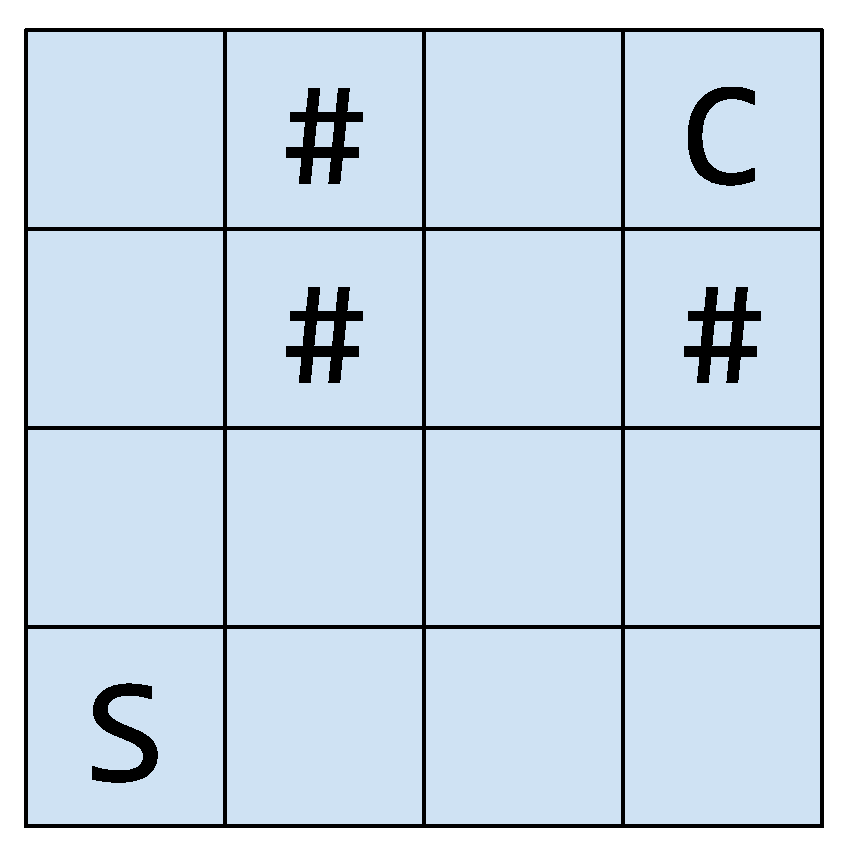
\includegraphics[width=4cm]{portals-example}
        \end{center}
    }

    \Scoring

    \begin{description}[leftmargin=0pt]
        \item[Deluppgift 1 (11 poäng):] $1 \le R \le 10, 1 \le C \le 10$.
        \item[Deluppgift 2 (20 poäng):] $1 \le R \le 50, 1 \le C \le 50$.
        \item[Deluppgift 3 (20 poäng):] $1 \le R \le 200, 1 \le C \le 200$.
        Varje öppen ruta har åtminstone ett väggblock bredvid sig.
        \item[Deluppgift 4 (19 poäng):] $1 \le R \le 200, 1 \le C \le 200$.
        \item[Deluppgift 5 (30 poäng):] $1 \le R \le 1000, 1 \le C \le 1000$.
    \end{description}

    \Constraints

    \begin{description}
        \item[Tidsgräns:] 1 s.
        \item[Minnesgräns:] 256 MB.
    \end{description}
\end{document}
